
\section{Week 5, Monday}

% \section{Perturbation Theory}

\subsection{Correlators in the Interacting Theory}

In quantum mechanics, perturbation theory is generally done in the
interaction picture where we split the Hamiltonian $H=H_0 +
H_\text{int}$ into a free Hamiltonian (harmonic oscillator of in some
disguise) and the interaction part $H_\text{int}$. The path integral
analog is to split the action
\begin{equation}
  S = S_0 + S_\text{int}
\end{equation}
into the action of a free particle and interactions. We use this split
to write correlators as
\begin{equation}
  \label{eq:corrSint}
  \langle 0 | T\mathcal{O} |0\rangle =
  \frac{
    \int \mathcal{D}\phi \; \mathcal{O} e^{i(S_0+S_\text{int})}
  }{ 
    \int \mathcal{D}\phi \; e^{i(S_0+S_\text{int})}
  }
  = 
  \frac{
    \langle0|T \mathcal{O} e^{iS_\text{int}} |0\rangle_0
  }{
    \langle0|T e^{iS_\text{int}} |0\rangle_0
  }
\end{equation}
where the subscript zero on $\langle \cdots \rangle_0$ means that we
use the free action $S_0$ only to compute the correlator. In
particular, this means that we can use Wick contractions to evaluate
the right hand side. For $\phi^4$ theory, the free and interacting
actions are the integrals over the Lagrange densities
\begin{equation}
  \mathcal{L}_0 = -\frac{1}{2} \partial_\mu \phi \partial^\mu \phi
  - \frac{1}{2} m^2 \phi^2
  , \quad
  \mathcal{L}_\text{int} = 
  - \frac{1}{4!} \lambda \phi^4
\end{equation}
The basic idea behind perturbation theory is to use the series
expansion
\begin{equation}
  e^{i S_\text{int}} = 
  1 + 
  \int d^4y \big(-\tfrac{i\lambda}{24} \phi^4 \big) + 
  \frac{1}{2!}
  \left[\int d^4y \big(-\tfrac{i\lambda}{24} \phi^4 \big)\right]^2
  + \cdots
\end{equation}
and compute correlators order-by-order in the coupling constant
$\lambda$. Note that the coupling constant is in both numerator and
denominator of eq.~\eqref{eq:corrSint}, so to first order we obtain
\begin{multline}
  \begin{split}
    \langle 0|T\mathcal{O}|0\rangle = &\;
    \sum_{n=0}^\infty \langle 0|T\mathcal{O}|0\rangle^{(n)} \lambda^n
    \\ &\;
    \langle 0|T\mathcal{O}|0\rangle_0 
    \\ &\;
    - \frac{i\lambda}{24} \int d^4y \Big(
    \langle 0|T\mathcal{O} \phi(y)^4 |0\rangle_0 - 
    \langle 0|T\mathcal{O} |0\rangle_0 
    \langle 0|T \phi(y)^4 |0\rangle_0 
    \Big)
    \\ &\;
    + O(\lambda^2)
  \end{split}
\end{multline}


\subsubsection{Leading Order Two-Point Function}

Let us start with the correlator of two fields. For simplicity, we
define the short-hand notation
\begin{equation}
  \phi_i = \phi(x_i)
  ,\quad
  \phi_y = \phi(y)
  ,\quad
  \langle \mathcal{O} \rangle = \langle 0|T \mathcal{O} |0\rangle
\end{equation}
Then the leading term in the expansions
\begin{equation}
  \langle \phi_1 \phi_2 \rangle = 
  \sum_{n=0}^\infty \lambda^n \langle \phi_1 \phi_2 \rangle^{(n)}
  \lambda^n
\end{equation}
is just the free field result
\begin{equation}
  \langle \phi_1 \phi_2 \rangle^{(0)}
  = 
  \langle \phi_1 \phi_2 \rangle_0
  = 
  \overline{\phi_1 \phi_2}
  = 
  \tfrac{1}{i} \Delta(x_1 - x_1)
\end{equation}
The following graphical notation will be useful in the future for Wick
contractions:
\begin{itemize}
\item Draw a point for each $x_i$, and
\item Connect two points with a line if the fields are Wick contracted.
\end{itemize}


\subsubsection{First-Order Two-Point Function}

The first order contribution is
\begin{equation}
  \langle \phi_1 \phi_2 \rangle^{(1)} = 
  - \frac{i}{24} \int d^4y \Big(
  \langle \phi_1 \phi_2 \phi_y^4 \rangle_0 - 
  \langle \phi_1 \phi_2  \rangle_0 
  \langle \phi_y^4 \rangle_0 
  \Big)
\end{equation}
The Wick contractions of the first term are
\begin{equation}
  \langle \phi_1 \phi_2 \phi_y^4 \rangle_0 = 
  3~
  \overline{\phi_1 \phi_2}~
  \overline{\phi_y \phi_y}~
  \overline{\phi_y \phi_y}
  + 
  12~
  \overline{\phi_1 \phi_y}~
  \overline{\phi_2 \phi_y}~
  \overline{\phi_y \phi_y}
\end{equation}
and the Wick contractions of the second term are
\begin{equation}
  \langle \phi_1 \phi_2 \rangle_0
  \langle \phi_y^4 \rangle_0 = 
  3~
  \overline{\phi_1 \phi_2}~
  \overline{\phi_y \phi_y}~
  \overline{\phi_y \phi_y}.
\end{equation}
The result is that
\begin{equation}
  \langle \phi_1 \phi_2 \rangle  =
  \overline{\phi_1\phi_2}
  - \frac{i\lambda}{2} \int d^4y\;
  \overline{\phi_1 \phi_y}~
  \overline{\phi_2 \phi_y}~
  \overline{\phi_y \phi_y} 
  + O(\lambda^2)
\end{equation}
The picture for the order-$\lambda$ term is what is called a tadpole: A
part of a diagram that is attached only through a single vertex. The
tadpole is divergent:
\begin{equation}
  \overline{\phi_y \phi_y} 
  = \tfrac{1}{i} \Delta(0)
\end{equation}
Going back to the path integral, we see that the problem arises when
translating the $\phi(y)^4$ in the action into a product of coincident
operators. Had we used normal ordering $:\phi_y^4:$, for example, then
the result would be finite. Equivalently, we could add
$\frac{i\lambda}{4}\Delta(0)\phi^2$ to the Lagrangian which also turns
out to cancel the divergent term. We will see how to deal with this
divergence systematically later.


\section{Week 5, Wednesday}

\subsubsection{Leading Order 4-Point Function}

The possible Wick contractions of the $4$ external positions $x_1$,
$\dots$, $x_4$ are just products of the leading $2$-point functions,
\begin{equation}
  \begin{split}
    \langle \phi_1 \phi_2\phi_3 \phi_4 \rangle 
    =&\;
    \langle \phi_1 \phi_2\phi_3 \phi_4 \rangle_0 + O(\lambda) 
    \\ =&\;
    \langle \phi_1 \phi_2 \rangle
    \langle \phi_3 \phi_4 \rangle +
    \langle \phi_1 \phi_3 \rangle
    \langle \phi_2 \phi_4 \rangle +
    \langle \phi_1 \phi_4 \rangle
    \langle \phi_2 \phi_3 \rangle +
    O(\lambda)
  \end{split}
\end{equation}


\subsubsection{First-Order 4-Point Function}

The order-$\lambda$ contribution to the 4-point correlator is
\begin{equation}
  \langle \phi_1 \phi_2 \phi_3 \phi_4 \rangle^{(1)} = 
  - \frac{i}{24} \int d^4y \Big(
  \langle \phi_1 \phi_2 \phi_3\phi_4 \phi_y^4 \rangle_0 - 
  \langle \phi_1 \phi_2 \phi_3 \phi_4  \rangle_0 
  \langle \phi_y^4 \rangle_0 
  \Big)
\end{equation}
The Wick contractions of the first term are
\begin{equation}
  \begin{split}
    \langle \phi_1 \phi_2 \phi_3 \phi_4 \phi_y^4 \rangle_0 =&\;
    24~
    \overline{\phi_1 \phi_y}~
    \overline{\phi_2 \phi_y}~
    \overline{\phi_3 \phi_y}~
    \overline{\phi_4 \phi_y}
    \\ &\;
    + 12\Big(
    \overline{\phi_1 \phi_2}~
    \overline{\phi_3 \phi_y}~
    \overline{\phi_4 \phi_y}~
    \overline{\phi_y \phi_y}
    + \text{perm.}
    \Big)
    \\ &\;
    + 3\Big(
    \overline{\phi_1 \phi_2}~
    \overline{\phi_3 \phi_4}~
    \overline{\phi_y \phi_y}~
    \overline{\phi_y \phi_y}
    + \text{perm.}
    \Big)
  \end{split}
\end{equation}
The Wick contractions of the second term just cancel the last summand
above (the terms multiplied by $3$). If you draw the corresponding
diagram, you see that they are ``vacuum bubbles'', that is, contain a
subdiagram that is disconnected from all external positions. Such
vacuum bubbles are generally divergent, though fortunately they end up
being subtracted off by the second term. 

We also notice that many of the terms are just products of 2-point
functions, for example
\begin{equation}
  \begin{split}
    \langle \phi_1 \phi_2 \rangle  \langle \phi_3 \phi_4 \rangle 
    =&\;
    \overline{\phi_1\phi_2}~
    \overline{\phi_3\phi_4}
    \\ &\;
    - \frac{i\lambda}{2} \int d^4y\;
    \Big(
    \overline{\phi_1 \phi_2}~
    \overline{\phi_3 \phi_y}~
    \overline{\phi_4 \phi_y}~
    \overline{\phi_y \phi_y} 
    +
    \overline{\phi_1 \phi_y}~
    \overline{\phi_2 \phi_y}~
    \overline{\phi_3 \phi_4}~
    \overline{\phi_y \phi_y} 
    \Big)
    \\ &\;
    + O(\lambda^2)
 \end{split}
\end{equation}
This should also not be surprising, part of amplitude for the
scattering process of two ingoing and two outgoing particles is just
two particles not interacting at all. In fact, only the single
connected diagram at $O(\lambda)$ remains after collecting everything
we can into products of two-point functions:
\begin{equation}
  \begin{split}
    \langle \phi_1 \phi_2\phi_3 \phi_4 \rangle 
    =&\;
    \langle \phi_1 \phi_2 \rangle
    \langle \phi_3 \phi_4 \rangle +
    \langle \phi_1 \phi_3 \rangle
    \langle \phi_2 \phi_4 \rangle +
    \langle \phi_1 \phi_4 \rangle
    \langle \phi_2 \phi_3 \rangle
    \\ &\;
    - i \lambda \int d^4y
    \overline{\phi_1 \phi_y}~
    \overline{\phi_2 \phi_y}~
    \overline{\phi_3 \phi_y}~
    \overline{\phi_4 \phi_y} 
    + O(\lambda^2)
  \end{split}
\end{equation}

In fact, this is true in general:
\begin{itemize}
\item Vacuum bubbles are cancelled by the expansion of the denominator 
  \begin{equation}
    \frac{1}{\int \mathcal{D}\phi e^{iS_\text{int}}},
  \end{equation}
  which we got because we are generally not able to normalize the path
  integral measure.
\item $n$-point correlators are sums of products of disconnected
  correlators plus the connected diagrams.
\item Each internal node is accompanied by a factor of $-i\lambda$ and
  an integral over its position. We will make these also part of the
  graphical notation.
\item Each term comes is multiplied with a combinatorial symmetry
  factor $\frac{1}{|\Aut G|}$, where $\Aut(G)$ is the automorphism
  group of the diagram. That is, count all ways to map the vertices to
  vertices and lines to lines. Note that we \emph{divide} by the
  number of automorphisms because each symmetry reduces the number of
  distinct Wick contractions we can make. In the diagrams so far, we had
  \begin{itemize}
  \item
    \begin{math}
      \overline{\phi_1 \phi_y}~
      \overline{\phi_2 \phi_y}~
      \overline{\phi_3 \phi_y}~
      \overline{\phi_4 \phi_y},
    \end{math}
    $\Aut G = 1$, coefficient $\tfrac{24}{24} = 1$,
  \item 
    \begin{math}
      \overline{\phi_1 \phi_y}~
      \overline{\phi_2 \phi_y}~
      \overline{\phi_y \phi_y},
    \end{math}
    $\Aut G = \mathbb{Z}_2$, coefficient $\tfrac{12}{24} = \tfrac{1}{2}$,
  \item 
    \begin{math}
      \overline{\phi_1 \phi_2}~
      \overline{\phi_y \phi_y}~
      \overline{\phi_y \phi_y},
    \end{math}
    $\Aut G = D_8$, that is, the dihedral group with $8$ elements,
    coefficient $\tfrac{3}{24} = \tfrac{1}{8}$.
  \end{itemize}
\end{itemize}


\subsection{Feynman Rules in Position Space}

\begin{definition}
  A Feynman graph in position space, for the $\phi^4$-theory, is a
  graph (undirected, without edge labels) with
  \begin{itemize}
  \item 1-valent vertices labelled by $x_i$, called ``external'',
  \item 4-valent vertices labelled by $y_j$, called ``internal'', and
  \item without vacuum bubbles.
  \end{itemize}
\end{definition}
In particular, disconnected graphs are allowed but each connected
component must be attached to at least one external vertex. As we have
seen, such a graph translates directly into a summand in the series
expansion of correlation functions. Explicitly, the rules are
\begin{definition}
  The Feynman rules for $\phi^4$-theory in position space are
  \begin{itemize}
  \item For each line joining two vertices $u$, $v$ multiply the
    integrand with a free propagator $\overline{\phi(u)\phi(v)} =
    \frac{1}{i} \Delta(u-v)$.
  \item For each vertex, integrate $-i\lambda \int d^4y_j$
  \item Multiply with the symmetry factor $\frac{1}{|\Aut G|}$.
  \end{itemize}
\end{definition}



\section{Week 5, Thursday}

\subsection{Feynman Rules in Momentum Space}

It turns out that the Feynman rules take a nicer for in momentum
space. Partly, this is because it is just more convenient for
accelerators where we scatter particles with fixed momentum. More
technically, recall that the Feynman propagator in position space is
quite complicated involving Bessel functions. And we have to compute
convolution integrals of the Feynman propagator because of the
$y_j$-integrals.

Hence, we apply Fourier transformation to each external position $x_i$
to obtain the $n$-point correlator in momentum space as
\begin{equation} 
  F(k_1, \dots, k_n) = 
  \int d^4x_1 \cdots 
  \int d^4x_n \;
  e^{i \sum_j k_j x_j}
  \langle \phi(x_1) \cdots \phi(x_n) \rangle.
\end{equation}
The Fourier transformation of just $\frac{1}{i}$ times the Feynman
propagator (i.e.\ the free field 2-point function) is
\begin{equation}
  \begin{split}
    G(k_1, k_2) =&\;
    \frac{1}{i}
    \int d^4x_1 \int d^4x_2\;
    e^{i( k_1 x_2 + k_2 x_2)}
    \int \frac{d^4k}{(2\pi)^4}
    \frac{e^{i k (x_1-x_2)}}{k^2 + m^2 -i\epsilon}    
    \\ =&\;
    \frac{1}{i}
    (2\pi)^4 \delta^4(k_1+k_2) \frac{1}{k_1^2 + m^2 - i\epsilon}.
  \end{split}
\end{equation}
For the vertex, note that its position $y$ occurs in the exponent of
the $4$ propagators that it is connected to. If we let $k_1$, $\dots$,
$k_4$ be the momenta in the $4$ propagators then the contribution of
the vertex boils down to
\begin{equation}
  -i \lambda \int d^4y \; e^{iy(k_1+k_2 + k_3 + k_4)}
  =
  -i \lambda (2\pi)^4 \delta^4(k_1+k_2 + k_3 + k_4).
\end{equation}
We notice that the delta functions just implement momentum
conservation on each line and each internal vertex. We make this part
of our graphical notation, and define
\begin{definition}
  A Feynman graph in momentum space for the $\phi^4$-theory is a graph
  with
  \begin{itemize}
  \item 1-valent external vertices labeled with inflowing
    $4$-momentum $k_j$,
  \item edges labelled by directed $4$-momenta $\ell_j$,
  \item 4-valent internal vertices, and
  \item without vacuum bubbles.
  \end{itemize}
\end{definition}
Each unique graph again can be translated into a particular summand in
the series expansion of the $n$-point correlator using 
\begin{definition}[Feynman rules]
  The Feynman rules for $\phi^4$-theory in momentum space are
  \begin{itemize}
  \item for each connected component with inflowing momenta $k_j$,
    multiply with $(2\pi)^4 \delta^4(\sum k_j)$,
  \item use momentum conservation along lines and vertices to replace
    internal momenta $\ell_j$ as far as possible,
  \item for each remaining internal momentum, integrate $\int
    \frac{d^4\ell}{(2\pi)^4}$,
  \item
    for each edge carrying momentum $k$, multiply the integrand with a factor
    $\frac{1}{i} \frac{1}{k^2+m^2-i \epsilon}$,
  \item for each 4-valent vertex multiply with $-i\lambda$,
  \item multiply with the symmetry factor $\frac{1}{|\Aut G|}$.
  \end{itemize}
\end{definition}
For example, for the tree graph $4$-point function with a single
internal vertex we get
\begin{equation}
  F^{(1)}_\text{conn} = 
  -i \lambda (2\pi)^4 \delta^4(k_1+k_2+k_3+k_4) \prod_{j=1}^4
  \frac{1}{k_j^2+m^2-i \epsilon}. 
\end{equation}
A more complicated diagram is the ``fish'', which has a $\mathbb{Z}_2$
symmetry:
\begin{multline}
  F = 
  \frac{1}{2}
  (-i\lambda)^2
  (2\pi)^4 \delta^4(k_1+k_2+k_3+k_4) 
  \prod_{j=1}^4 \frac{1}{k_j^2+m^2-i \epsilon}
  \\
  \times
  \int \frac{d^4\ell}{(2\pi)^4}~
  \frac{1}{\ell^2 + m^2 -i\epsilon}~
  \frac{1}{(k_1+k_2-\ell)^2 + m^2 -i\epsilon}
\end{multline}
There is a $4$-dimensional momentum integration, but the integrand
only falls off like $\ell^{-4}$. This results in a logarithmic
divergence if you try to do the momentum integral. Because it appears
at high energies, this is called a UV divergence. We will have to
understand how to systematically deal with these.

If $m^2=0$ and, $k_1=-k_2$, then there is in addition a divergence as
$\ell\to 0$. Such a divergence is called an IR divergence. It
typically appears for special values of the external momenta, whereas
the UV divergence is independent of the external momenta. In the
following, we will only consider $m^2\not=0$, so at least we do not
have any problems with IR divergences.



\subsection{Power Counting}

Counting the powers of the momenta in the integral gives us a first
hint at whether there is a UV divergence, so we want to do it more
systematically for all diagrams. So let us define the counts of the
constituents of a Feynman graph as
\begin{itemize}
\item $V$ = number of (internal) vertices,
\item $I$ = number of internal lines,
\item $E$ = number of external lines.
\end{itemize}
Each internal line ends at two vertices, each external line ends at
one vertex. Since the vertices are 4-valent, we get
\begin{equation}
  4V = 2I + E.
\end{equation}
The number of loops $L$ equals the number of unconstrained internal
momenta. We get one from each internal line, but can eliminate $V-1$
using all momentum conservation rules except for the overall momentum
conservation. Hence,
\begin{equation}
  L = I - (V-1) = I - V + 1.
\end{equation}
We now define the superficial (apparent) degree of divergence $D$ as
the overall power of the momentum in the integral. For reasons that
will be clear later, we want to do it in arbitrary space-time
dimension $d$. Then we get $Ld$ powers of the momentum from the
measure of the $L$ integrals, and we get a inverse momentum squared
from each internal propagator. Hence, the degree of divergence is
\begin{equation}
  D = dL - 2I
\end{equation}







\section{Week 6, Monday}

We simplify the superficial degree of divergence to 
\begin{equation}
  \begin{split}
    D =&\; dL - 2I
    \\ =&\;
    d - \frac{d-2}{2}E + V(d-4)
    \\ =&\;
    \begin{cases}
      4-E & \text{in 4d} \\
      2-2V & \text{in 2d}.
    \end{cases}
  \end{split}
\end{equation}
A superficial divergence (by power counting) does not necessarily
translate into an actual divergence, for example the tree level
interaction (E=4, V=1) has superficial degree of divergence
$D=0$. But, since there is no loop integral, it obviously does not
diverge logarithmically. Neither does a superficial convergence $D<0$
guarantee convergence, for example attach a tadpole to any convergent
diagram. The tadpole integral remains divergent. But in that case the
divergence just comes from a sub-diagram, it is not inherently due to
the larger diagram. This suggests that we should only look at diagrams
without superficially divergent sub-diagrams; If there is a divergent
sub-diagram then you really only have to worry about that
sub-diagram. This suggests the following:
\begin{theorem}[Dyson-Weinberg convergence theorem]
  A superficially convergent diagram such that all of its sub-diagrams are
  also superficially convergent is actually convergent.
\end{theorem}
The theorem might seem obvious but is actually rather tricky due to
the issue of overlapping divergences. We will explain what this in a
second, but first let us classify the primitively divergent diagrams
in $\phi^4$-theory. That is, look for the divergent diagrams that do
not have a divergent sub-diagram. These are the real troublemakers,
and we really only have to deal with their divergences.
\begin{itemize}
\item In the two-dimensional $\phi^4$-theory there is only a single
  primitively divergent diagram, namely the tadpole. It has
  superficial degree of divergence $D=0$.
\item In the four-dimensional $\phi^4$-theory there are two primitive
  divergences at $O(\lambda)$, namely the tadpole $D=2$ and the
  ``fish'', the only (up to permutations of the external vertices)
  connected one-loop diagram contributing to the 4-point
  function. There are further primitive divergences at all higher
  powers of $\lambda$, but only with two or four external legs.
\item In the four-dimensional $\phi^k$-theory with $k\geq 5$ there are
  primitive divergences with any number of external legs. This is what
  makes the theory non-renormalizable, as we will see.
\end{itemize}


\subsection{Overlapping Divergences}

There is one subtlety when dealing with potentially divergent loop
integrals: Sometimes you can't split the integrals into an outer
integral times an inner integral and analyze the convergence
separately. This happens when an internal line is part of two separate
loops, giving rise to a propagator $\frac{1}{(\ell+p)^2+m^2}$ that
depends on both the $\ell$ and $p$-loop momentum. More properly, these
should be called overlapping integrals.

The simplest overlapping loop diagram would be in $\phi^3$-theory.
So, just for this section, let us consider tri-valent interaction
vertices and the diagram
\begin{center}
  {\fmfframe(8,0)(8,0){
      {
        \begin{fmffile}{figures/fig-overlapping-divergence}
          \begin{fmfgraph*}(200,50)
            \fmfleft{left}
            \fmfright{right}
            \fmftop{top}
            \fmfbottom{bottom}
            \fmf{plain_arrow,tension=4}{left,x1}
            \fmf{plain_arrow,tension=4}{right,x2}
            \fmf{plain_arrow,label=$p$,label.side=left}{x1,top}
            \fmf{plain_arrow,label=$\ell$,label.side=right}{x2,top}
            \fmf{plain}{x1,bottom}
            \fmf{plain}{x2,bottom}
            \fmf{plain_arrow,label=$p+\ell$}{top,bottom}
            \fmflabel{$k_1$}{left}
            \fmflabel{$k_2$}{right}
          \end{fmfgraph*}
        \end{fmffile}}
    }}
\end{center}
leading to the loop integral
\begin{equation}
  \begin{split}
    I =&\; \int 
    d^4p \;
    d^4\ell \;
    \frac{1}{p^2+m^2-i\epsilon}
    \frac{1}{\ell^2+m^2-i\epsilon}
    \\ &\; \qquad
    \times
    \frac{1}{(p+\ell)^2+m^2-i\epsilon}
    \frac{1}{(p-k_1)^2+m^2-i\epsilon}
    \frac{1}{(\ell-k_2)^2+m^2-i\epsilon}
  \end{split}
\end{equation}
where we left out constants and the external propagators, anything
that does not depend on the loop momenta. We now
\begin{itemize}
\item Perform Wick rotation: drop the $-i\epsilon$.
\item Set $m^2=0$ and $k_1=0=k_2$ since the UV divergence is at $k^2
  \gg m^2, k_1^2, k_2^2$.
\item Remove a region of small momenta by hand to avoid the IR
  divergence.
\end{itemize}
Hence the asymptotic behavior of the loop integral is that of 
\begin{equation}
  I \sim
  \int \frac{d^4p \; d^4\ell}{p^4 (p+\ell)^2 \ell^4}.
\end{equation}
This is an example of an overlapping divergence: by power counting,
the diagram superficial degree of divergence $D=2\times 4-5\times 2
=-2$ and no divergent sub-diagram, so we expect convergence. But the
actual integral is not so obviously convergent, for example there is a
region where $p+\ell$ is constant. In that region, just the
$p$-integral seems to have superficial degree of divergence $D=0$,
which would indicate a logarithmic divergence. This is actually not
true, the whole integral still converges.

To show that the integral does converge, we have to split up the
domain according to which momentum factor is the smallest. For
example, consider the region where $\ell^2$ is the smallest,
\begin{equation}
  U_p = \big\{
  p \big|
  p^2 \geq \ell^2,~ (p+\ell)^2 \geq \ell^2  \big\},
\end{equation}
and combine it with the necessary IR cutoff
\begin{equation}
  U_\ell = \big\{
  \ell \big| \ell^2 \geq 1 \big\}.
\end{equation}
Splitting the 4-momentum $\ell = \bar\ell e_\ell$ into its absolute
value $\bar\ell\in\R$ and unit 4-vector $e_\ell$, the loop integral
becomes
\begin{equation}
  I \sim
  \int_{U_p} \int_{U_\ell}
  \frac{d^4p \; d^4\ell}{p^4 (p+\ell)^2 \ell^4}
  = 
  \int_0^\infty d\bar\ell
  \bar\ell^3
  \frac{1}{\bar\ell^6}
  \int_{S^3} de_\ell 
  \int_{U_{p'}}
  \frac{d^4 p'}{(p')^4 (p'+e_\ell)^2}
\end{equation}
where we rescaled $p' = p \bar\ell$ and integrate over the  rescaled
region
\begin{equation}
  U_{p'} = \big\{
  p' \big|
  (p')^2 \geq 1,~ (p'+\ell)^2 \geq 1  \big\}.
\end{equation}
The $\bar\ell$-integration is, indeed, of superficial degree of
divergence $D=-2$. The overlapping diagram does converge as expected
by power counting, the potential overlapping divergence does not cause
an actual divergence.



\section{Week 6, Wednesday}


\subsection{Regularization}

As we have seen, it is unavoidable that some of the Feynman diagrams
contain divergent momentum integrals. It turns out that this can be
dealt with, but we must be careful when handling the
infinities. Naively, $1+\infty = \infty$ so how can we make any
sensible computation? The key is to introduce a suitable parameter
(called ``regulator'') that makes all loop integrals finite. Perhaps
the simplest way to do that is to cut off momentum integrals at some
scale $\Lambda$, for example for the tadpole integral
\begin{equation}
  A(\Lambda) = - \frac{\lambda}{2} \int_{|\ell| \leq \Lambda}
  \frac{d^4 \ell}{\ell^2+m^2}.
\end{equation}
Only at the end we then let $\Lambda \to \infty$ to recover the
integration over the entire momentum space. This is actually very
similar to the lattice computation that we have seen before, there the
lattice spacing $a$ also ensures that we can only sample waves with
momentum up to some upper limit $\approx \frac{1}{a}$.

Both the direct momentum cutoff and the lattice regularization break
Lorentz invariance badly: Cutting off momenta in some special frame
breaks boost invariance. And the lattice even breaks rotational
invariance down to a discrete subgroup, namely rotations by
$\tfrac{2\pi}{4}$. Since symmetries are one of the key guiding
principles in physics, a lot of attention was spent on finding
regularization schemes that do not break a particular symmetry that
one is interested in. One such example is analytic regularization
\begin{equation}
  A(z) = - \frac{\lambda}{2} \int
  \frac{d^4 \ell}{\big(\ell^2+m^2\big)^z},
  \quad
  z \gg 1.
\end{equation}
However, the most common regularization scheme is dimensional
regularization where we compute the momentum integral in $d-\omega$
dimensions for some $\omega > 0$. This is the regularization scheme
that we will always be using in the following. For example, the
tadpole integrand is actually rotationally symmetric so we can just
split it into a one-dimensional integral times the area of the
$(d-\omega)$-sphere.

In each integral dimension $d\in \Z$, the volume of the
$d$-dimensional disk and the area of the $d$-dimensional sphere are
related by the recurrence relations for the area of the
$d$-dimensional disc $D_d$ and sphere $S_d$,
\begin{equation}
  D_d = \frac{1}{d} S_{d-1}
  ,\quad
  S_d = 2\pi D_{d-1},
\end{equation}
which have a simple geometric origin. We can solve them in closed form
as
\begin{equation}
  D_d = \frac{\pi^{d/2}}{\Gamma(\frac{d}{2}+2)}
  ,\quad
  S_{d-1} = \frac{2 \pi^{d/2}}{\Gamma(\frac{d}{2})}.
\end{equation}
The result is actually an analytic function of the dimension, and we
will use it to define what me mean by the area of the $(d-1)$-sphere
for arbitrary $d\in\mathbb{C}$. It is by no means the unique analytic
function that equals $S_{d-1}$ when restricted to the integers, but it
is certainly the most convenient choice. Any other choice would just
be a different regularization scheme.

Hence, the dimensionally-regulated tadpole is 
\begin{equation}
  A(\omega) = -\frac{\lambda}{2}
  \int
  \frac{d^{d-\omega}\ell}{(2\pi)^{d-\omega}} ~
  \frac{1}{\ell^2 + m^2}
  = -\frac{\lambda}{2}
  S_{d-1-\omega}
  \int_0^\infty \frac{d\bar\ell ~ \bar\ell^{d-1-\omega}}{\bar\ell^2 + m^2}.
\end{equation}
The remaining one-dimensional integral can be solved by the formula
\begin{equation}
  \int_0^\infty 
  \frac{x^k dx}{\big(x^n + a^n\big)^r} 
  =
  \frac{
    (-1)^{r-1}\; \pi \; a^{k+1-nr} \; \Gamma\big(\tfrac{k+1}{n}\big)
  }{
    n \; \sin\big(\tfrac{k+1}{n} \pi\big) 
    \; \Gamma\big(\tfrac{k+1}{n}-r+1\big) 
    \; (r-1)!
  }
\end{equation}
and using Euler's reflection formula
\begin{equation}
  \Gamma(x) \Gamma(1-x) = \frac{\pi}{\sin(\pi x)}.
\end{equation}
The result is 
\begin{equation}
  A(\omega) = -\frac{\lambda}{4\pi} 
  \Gamma\big(\tfrac{\omega}{2}\big)
  \left(\frac{2 \sqrt{\pi}}{m} \right)^\omega,
\end{equation}
but there is something troubling about the $m^{-\omega}$: what kind of
units (or mass dimension) does such a quantity have? The answer is
that we forgot that the mass dimension of $\lambda$ is also
non-trivial and dependent on the ambient space dimension. In
particular, in $d-\omega$ dimensions we have $[\lambda] =
2+\omega$. To better understand how the units work in the equation, it
is convenient to split the dimensionful coupling constant
\begin{equation}
  \lambda = \lambda_0 M^{2+\omega}
\end{equation}
into a dimensionless coupling constant $\lambda_0$ times a mass scale
$M$. Then,
\begin{equation}
  A(\omega) = -\frac{\lambda_0 M^2}{4\pi} 
  \Gamma\big(\tfrac{\omega}{2}\big)
  \left(\frac{2 \sqrt{\pi}M}{m} \right)^\omega,
\end{equation}
At the end of the day, we will of course be interested in the limit
$\omega\to 0$, and we can understand the behavior of $A(\omega)$ in
this limit by expanding it in a Laurent
series. Using\footnote{$\gamma\approx 0.577\dots$ is the
  Euler-Mascheroni constant}
\begin{equation}
  \Gamma(\omega) = \frac{1}{\omega} - \gamma + O(\omega)
  ,\quad
  x^\omega = 1 + \omega \ln(x) + O(\omega^2)
\end{equation}
we obtain
\begin{equation}
  A(\omega) = -\frac{\lambda_0 M^2}{4\pi}
  \left[
    \frac{2}{\omega}
    - \gamma
    + \ln\left(
      \frac{4\pi M^2}{m^2}
    \right)
    + O(\omega)
  \right]
\end{equation}
Clearly this is still infinite in the limit $\omega\to 0$, as it
must. But the infinity just comes from the simple pole at $\omega=0$,
so we can easily handle it.



\subsection{Renormalization}

We did not write the external propagators in the previous section for
brevity, this is also called the amputated Feynman diagram. The actual
contribution to the two-point function is
\begin{equation}
  A(\omega) \delta(k_1-k_2) \frac{1}{k_1^2+m^2} ~ \frac{1}{k_2^2+m^2}.
\end{equation}
To get rid of the $\frac{1}{\omega}$ pole, we now add a new Feynman
rule that cancels it. The easiest way is to add a new 2-valent vertex
with just the right interaction strength such that 
\begin{equation}
  \raisebox{-1mm}{\fmfframe(8,0)(8,0){
      {
        \begin{fmffile}{figures/fig-counterterm}
          \begin{fmfgraph*}(80,10)
            \fmfleft{left}
            \fmfright{right}
            \fmf{plain}{left,center,right}
            \fmfv{decoration.shape=cross}{center}
            \fmflabel{$k_1$}{left}
            \fmflabel{$k_2$}{right}
          \end{fmfgraph*}
        \end{fmffile}}
    }}
  ~= 
  \frac{\lambda_0 M^2}{4\pi}
  \left(\frac{2}{\omega} + F \right)
  \delta(k_1-k_2) \frac{1}{k_1^2+m^2} ~ \frac{1}{k_2^2+m^2},
\end{equation}
where $F$ is some arbitrary finite quantity. Then the
$\frac{1}{\omega}$-pole cancels in sum of the tadpole and the
counterterm, rendering the 2-point correlator finite at order
$O(\lambda)$. Of course we cannot just add new Feynman rules at will,
they must come from an interaction term in the Lagrangian. Since the
counterterm vertex is 2-valent, it is the Feynman rule corresponding
to the interaction term
\begin{equation}
  \mathcal{L}_\text{ct} = 
  \frac{1}{2} ~
  \frac{\lambda_0 M^2}{4\pi} 
  \left(\frac{2}{\omega} + F \right) \phi^2
\end{equation}



\section{Week 6, Thursday}

\subsection{Two-Point Correlators at Second Order}

Up to $O(\lambda^2)$, the Feynman rules including the counterterm
yield
\begin{itemize}
\item Tree level propagator $\frac{1}{k^2+m^2}$,
  \begin{center}
    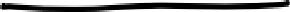
\includegraphics[scale=0.7]{figures/draw-propagator-tree.pdf}
  \end{center}
\item At $O(\lambda)$: Tadpole + counterterm.
  \begin{center}
    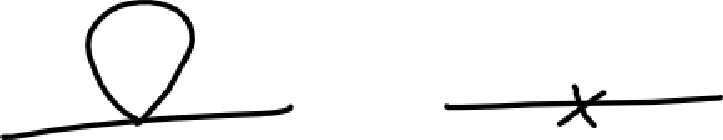
\includegraphics[scale=0.7]{figures/draw-propagator-tadpole_and_counterterm.pdf}
  \end{center}
\item Four one-particle reducible diagrams, and
  \begin{center}
    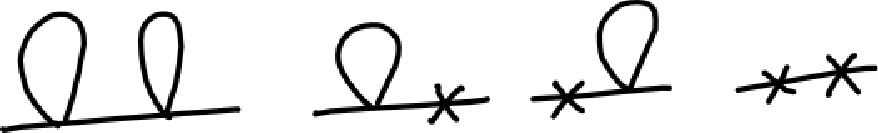
\includegraphics[scale=0.7]{figures/draw-propagator-twoloop_reducible.pdf}
  \end{center}
\item Three one-particle irreducible diagrams.
  \begin{center}
    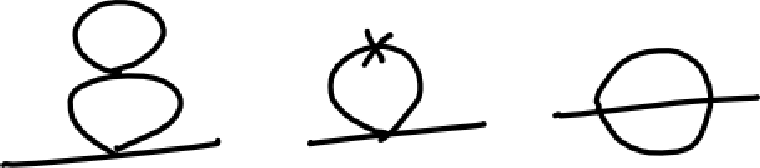
\includegraphics[scale=0.7]{figures/draw-propagator-twoloop_1PI.pdf}
  \end{center}
\end{itemize}
By one-particle irreducible diagram (1PI) we mean any diagram that can
not be disconnected by cutting a single internal line. Like the
disconnected diagrams, the one-particle reducible diagrams are again a
type of diagram that we have to add up to get the correlation
function, but that really is just a combination of lower-order
diagrams and does not present any real difficulty. In particular, up
to a factor of the external propagator $\frac{1}{k^2+m^2}$, the sum of
the four one-particle reducible diagrams is just the square of tadpole
and counterterm.

The really interesting part are the three 1PI diagrams. The ``double
scoop'' (first) diagram is divergent only because the top loop
integral is a tadpole, so it yields the same $A(\omega)$ as the
tadpole times whatever the convergent integral over the lower loop
is. To it, we have to add the tadpole-with-counterterm (second)
diagram. Its loop integral is just the same as the lower loop integral
of the previous diagram, now multiplied by the counterterm. Hence, the
first two diagrams just cancel the $\frac{1}{\omega}$ pole just like
tadpole and counterterm alone. Finally, the ``sunset'' diagram (third)
is convergent in two dimensions.

By as similar reasoning, the addition of the counterterm to the
Feynman rules always cancels the $\frac{1}{\omega}$ pole from any
tadpole sub-diagram, rendering every correlation function finite. As a
word of warning, however, this is not typical of quantum field
theories. For example in 4-d $\phi^4$-theory, there are new
divergences at each order in $\lambda$, for which we have to add more
and more counterterms. In particular, the leading
$\frac{1}{\omega^2}$-divergence will cancel between the first two
diagrams as above, but only to leave a $\frac{1}{\omega}$-pole that
still diverges. However, as we will see, the $\phi$-dependence of all
of the counterterms is just like one of the terms that is already in
the Lagrangian, and this is what makes the theory renormalizable.


\subsection{Renormalization Prescription}

To summarize, we can combine the Lagrangian and counterterms into a
renormalized Lagrangian
\begin{equation}
  \mathcal{L}_\text{Ren} = 
  -\frac{1}{2} \partial_\mu \phi \partial^\mu \phi
  -\frac{1}{2} m_\text{bare}^2 \phi^2 
  - \frac{1}{4!} \lambda_\text{bare} \phi^4
\end{equation}
with ``bare'' parameters
\begin{equation}
  \begin{split}
    \lambda_\text{bare} =&\; \lambda_0 M^2 = \lambda \\
    m_\text{bare}^2 =&\; 
    m^2 - \frac{\lambda_0 M^2}{4\pi} \left( \frac{2}{\omega} + F\right)
  \end{split}
\end{equation}
The bare parameters in the Lagrangian are unphysical (and usually
infinite in the $\omega\to 0$ limit). We can now compute correlation
functions in two ways, either using the renormalized Lagrangian and
bare parameters or using the original Lagrangian with (divergent)
counterterms. Either way, the divergences in the $\omega\to 0$ limit
cancel to give finite correlation functions
\begin{equation}
  \Gamma_{\mathcal{L}_\text{Ren}}
  (k_1, \dots, k_n; m_\text{bare}^2, \lambda_\text{bare}, \omega) = 
  \Gamma_{\mathcal{L}+\mathcal{L}_\text{ct}}
  (k_1, \dots, k_n; m^2, \lambda_0, M, \omega).
\end{equation}
Analyzing the $M$-dependence of this equation will lead us to the
renormalization group later, but before we get there we need to
understand how to relate the parameters to the physical mass and
coupling strength.

Really, the mass and coupling constant are experimental input. Because
of the ambiguities introduced in the renormalization procedure, these
are not directly related to any set of parameters in the
Lagrangian. Instead, we have to fix a certain number of observables
and match the computed value (as a power series in the coupling
constant, most likely) to the experimental input. The ambiguity in
choosing a particular set of observables is called the
``renormalization prescription'', and reflects the ambiguity in the
finite part of the counterterms.

In quantum field theory, the observables are simply the correlation
functions. The renormalization prescription for the mass are always
linked to the two-point functions in some way. Popular choices are
\begin{itemize}
\item Pole mass: Let the mass be the location of the pole in the
  two-point function $\Gamma^{(2)}$ in Minkowski space. This is a very
  physical prescription, but not convenient in Euclidean space after
  Wick rotation.
\item More convenient for calculations (as long as there is no IR
  divergence) is to demand that
  \begin{equation}
    \frac{1}{\Gamma^{(2)}(k_1,k_2)} \Big|_{k_1=k_2=0} = m^2.
  \end{equation}
  This is just a little bit unphysical as $k_1=k_2=0$ is not really
  allowed for massive external particles, it violates the mass shell
  condition. But nothing stops us from evaluating the $2$-point
  function and use it in our prescription. Inverting the two-point
  function to first order in $\lambda$ is easy enough, and by summing
  the tree-level, tadpole, and counterterm we obtain
  \begin{equation}
    \frac{1}{\Gamma^{(2)}(k_1,k_2)} \Big|_{k_1=k_2=0} =
    m^2 \left[
      1 + 
      \frac{\lambda_0 M^2}{4\pi m^2} \left(
        -\gamma + 
        \ln\left(\frac{4\pi M^2}{m^2}\right) - F
      \right)
      + O(\lambda^2)
    \right]
  \end{equation}
  which we can solve by setting
  \begin{equation}
    F = -\gamma + \ln\left(\frac{4\pi M^2}{m^2}\right)
  \end{equation}
\item Even more convenient for calculations is the ``minimal
  subtraction'', where we set $F=0$ as our choice of renormalization
  prescription. In other words, we only use the minimial counterterm
  necessary to precisely cancel the $\frac{1}{\omega}$-pole.
\end{itemize}


